\chapter{Introduction}
	\label{chap:intro}
	
	\section{Current State of Mobile Cyber Security}
		\label{sec:intro_motivation} 
		
		Ever since the release of the iPhone in 2007, mobile devices have played an increasingly larger role in our lives. We are using mobile devices for education, mobile banking, entertainment, work, and more. Moreover, 52.6 percent of global web traffic came from mobile devices in 2019, up from 31.6 per cent in 2015 \cite{statista_mobile_web_traffic}. 
		
		Meanwhile, the cyber security of mobile apps is underwhelming. A 2018 study done by cyber security consultancy Positive Technologies analysed 17 mobile apps, 8 for Android and 9 for iOS \cite{pt_mobile_apps_2019}. It found that only 11\% of the apps had an acceptable level of security, with 56\% having a below-average level of security, and 43 percent of Android apps had critical vulnerabilities. A more worrying piece of information is that the average Android client app in the study contained 3.7 vulnerabilities, of which 1.1 were of high-risk \cite{pt_mobile_apps_2019}.
		
		Against the lacklustre security of mobile apps, attackers are becoming more relentless and are using more elaborate techniques \cite{pt_threatscape_2018}. In figure \ref{fig:no_attacks_evolution} you can see how the monthly number of reported cyber attacks has increased since 2017.
		
		\begin{figure}[h]
            \centering
            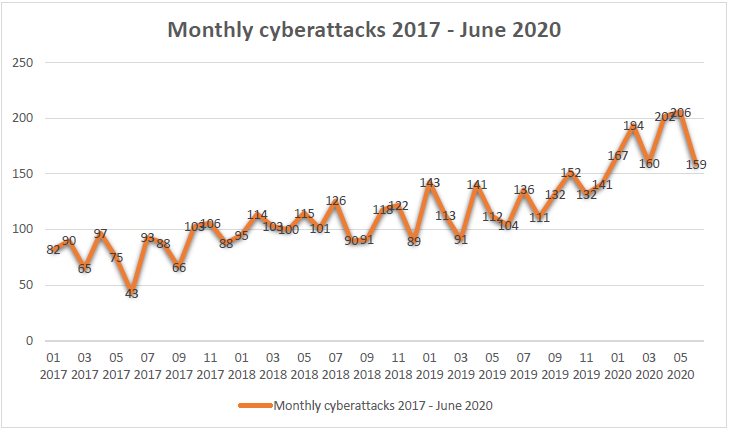
\includegraphics[width=0.5\textwidth]{graphics/threatscape_chart.PNG}
            \caption{Increasing number of monthly cyber attacks since 2017. Data is compiled from \cite{pt_threatscape_2018}, \cite{pt_threatscape_2019}, \cite{pt_threatscape_2020} and              \cite{pt_threatscape_2020q2}.}
            \label{fig:no_attacks_evolution}
        \end{figure}
		
        Concurrently, Android app security is not improving. A study conducted on over 400,000 APKs released between 2010 and 2016 belonging to over 28,000 apps analyzed how security has evolved over time \cite{android_vulnerabilities_evolution}. It discovered that critical vulnerabilities of various types have always been common in apps. Moreover, app updates generally do not improve security, and can even re-introduce previously fixed vulnerabilities. This is the largest and most comprehensive study to date. Another study found that the proportion of malware has dropped significantly in 2017 compared to 2014 \cite{newer_android_vulnerabilities_evolution}, though it studied fewer APKs than \cite{android_vulnerabilities_evolution}.
		
	\section{Motivations}
	    \label{sec:intro_motivations}
	    
	    We chose to explore Inter Component Communication vulnerabilities in Android for reasons based on the current state of mobile application security and how this vulnerability category is touched upon in related work.
	    
	    \subsection{ICC-related vulnerabilities in current mobile apps}
	        \label{subsec:ICC_vulnerabilities_current_apps}
	    
    	One of the categories of vulnerabilities that the authors of \cite{pt_mobile_apps_2019} analysed was Inter Component Communication vulnerabilities. Android components are the logical building blocks of an app, and components can communicate with other components, of the same app or of other apps on the same device.
    	
    	In the study conducted in \cite{pt_mobile_apps_2019}, 29 percent of client apps used insecure inter-process communication, and the average Android app had 1.1 ICC-related vulnerabilities \cite{pt_mobile_apps_2019}. Insecure inter-component communication is a high-risk vulnerability, and it is more dangerous than insecure storage or other common vulnerabilities \cite{pt_mobile_apps_2019}, and therefore deserves attention from developers and cyber security specialists.
		
		Moreover, while the overwhelming majority of vulnerabilities of other types are introduced in apps through the use of third-party libraries and rarely through developer code, ICC vulnerabilities differ in this regard. According to \cite{android_vulnerabilities_evolution}, between a third and a half of ICC vulnerabilities come from code written by the developer directly. Therefore, education regarding this type of vulnerability addressed to the average developer would greatly help with minimizing the occurrence of these faults.
		
		Finally, the reality is that software developers are not always trained in cybersecurity, may lack costly automatic analysis tools, or do not have the time to design and implement secure software due to tight deadlines \cite{malwarebytes_blog}. Therefore, there needs to be more awareness of cyber security in the software development industry, especially among developers.
		
		\subsection{ICC-related vulnerabilities in related work}
		    \label{subsec:ICC_related_work}
		
		Vulnerabilities and cyber attacks concerning communication between Android components are not showcased in detail or intuitively in real-world projects similar to mine.
		
		Damn Insecure and Vulnerable App has challenges 9 and 10 that show examples of hijacking intents meant for a vulnerable activity. DIVA also contains challenge 11 where a malicious user can send intents to extract data from an unprotected content provider \cite{diva_walkthrough}. 
		
		Purposefully Insecure and Vulnerable Android Application, also called PIVAA from here on, has three challenges on components that are insecurely exported and thus can be sent malicious intents. The challenges show this vulnerability in a broadcast receiver, a service, and a content provider, respectively.
		
		Another intentionally insecure Android app used for educational purposes is InsecureBankv2 \cite{android_insecure_bank_github}. Similar to PIVAA, it contains vulnerable components that can be started by a malicious app with a specially crafted intent, though it has a vulnerable activity, broadcast receiver, and content provider and no service, unlike PIVAA \cite{android_insecure_bank_walkthrough}. Furthermore, another ICC-related vulnerability it contains is intent hijacking, which allows malware to intercept intents sent by components of the vulnerable app.
		
		Damn Vulnerable Web Application, an intentionally insecure web application with vulnerabilities such SQL injection or Cross-Site Scripting, does not cover any Inter Process vulnerabilities. TryHackMe.com is an interactive website for learning cyber security and penetration testing. Although easy to use and very useful, it has no dedicated activities on Android ICC.
		
		None of the projects mentioned in this subsection cover all types of ICC vulnerabilities. Furthermore, DIVA, PIVAA, and InsecureBankv2 only offer one application that has various components for each vulnerability they implement, they do not offer standalone apps for each vulnerability. More importantly, these applications need to be used together with ADB shell on a computer to perform each attack. Thus, these projects do not offer real examples of malicious apps. On top of that, they provide little to no instructions and do not show detailed explanations and code examples of the vulnerability and how to fix it. Finally, they do not provide much interactivity and some of the apps contain major UI bugs, such as the About project activity in PIVAA.
		
		Damn Vulnerable Web Application, or DVWA, had multiple security levels for each vulnerability, where in each one the vulnerable program uses increasingly secure code. It tells the user what each level does, how secure it is, and shows relevant source code for it. This is a very useful feature that is not shared by the three insecure Android app projects mentioned earlier in this subsection.
		
	\section{Project Aims and objectives}
		\label{sec:intro_objective} 
    	
    	This project aims to create an educational tool that explores vulnerabilities related to insecure Inter Component Communication in Android, that can be used by penetration testers and developers. This tool should teach users about ICC vulnerabilities and attacks in Android apps and raise awareness.
        
        The primary objectives of the project, that make up the minimal viable product, are:
        
        \begin{itemize}
            \item Develop a home application through which the user can access all educational material and can interactively learn about each vulnerability and how to exploit it and fix it.
            \item Develop a series of apps that act as either a vulnerable app or a malicious app. Each challenge has two apps, a vulnerable app and a malware that exploits the former.
            \item Make sure that the experience of using the product is cohesive and pleasant.
        \end{itemize}
	
	\section{Contributions} 
		\label{sec:intro_contributions} 
		
		The main contributions of this project are as follows:
		
		\begin{itemize}	
		
			\item \textbf{An intentionally insecure Android image focused on Inter Component Communication vulnerabilities and attacks}
			
			\item \textbf{An educational tool for Android vulnerabilities that does not require the use of ADB shell and can be used on one's smartphone}
			
			\item \textbf{An intentionally insecure Android image which includes malware:}
			Unlike existing projects of this type, we have developed real malware apps that attack other apps in the image.
			
			\item \textbf{An intentionally insecure Android image with multiple security levels for each vulnerability, like DVWA has:}
			No other related work on Android except ours implements this, to our knowledge.
			
		\end{itemize}